\documentclass{article}
\usepackage[]{circuitikz}
\usepackage{tikz}
\usepackage{color}
\usepackage{lscape}
\begin{document}	
%\begin{landscape}	
\newcommand{\speaker}[2] % #1 = name from to[generic,n=#1], #2 = rotation angle
{\draw[thick,rotate=#2] (#1) +(.2,.25) -- +(.7,.75) -- +(.7,-.75) -- +(.2,-.25);}

%%%%%%%%%%%%%%%%%%%% task 2a fig 1 %%%%%%%%%%%%%%%%%%%%

\begin{circuitikz}[scale = 2, transform shape, american voltages, line width=1.5pt]

	\draw 
	(0, 0) node[ground]{} to [vC, l=$C_{pixel}$] ++(0, 5);
	
	\draw
	(1,5) node[spdt] (s1) {}
	(0,5) -- (s1.in) ;
	
	\draw (s1.out 1) -| node[rground,yscale=-3](5V){} ++(1,1);
	\draw (5V) node[left=0em,above=3.5em,anchor=south] {$5V (V_{DD})$};
	
	\draw (s1.out 2) -- ++(1,0) node(compp1){} to [C, l=$C_{fixed}$] ++(0,-4.65) node[ground]{};
	
\end{circuitikz}

%%%%%%%%%%%%%%%%%%%% task 2a fig 2 %%%%%%%%%%%%%%%%%%%%
\newpage
\begin{circuitikz}[scale = 2, transform shape, american voltages, line width=1.5pt]
	% The top line plus the voltage
	\draw 
	(0, 0) node[ground]{} to [vC, l=$C_{pixel}$] ++(0, 5);
	
	\draw
	(1,5) node[spdt, yscale=-1] (s1) {}
	(0,5) -- (s1.in) ;

	
	\draw (s1.out 2) -| node[rground,yscale=-3](5V){} ++(1,1);
	\draw (5V) node[left=0em,above=3.5em,anchor=south] {$5V (V_{DD})$};
	
	\draw (s1.out 1) -- ++(1,0) node(compp1){} to [C, l=$C_{fixed}$] ++(0,-4.65) node[ground]{};
	\draw (compp1) to[short, -o] ++(1,0) node(Vx){};
	\draw (Vx) node[anchor=south] {$V_x$};
	
\end{circuitikz}

%%%%%%%%%%%%%%%%%%%% task 2a fig 3 discharge %%%%%%%%%%%%%%%%%%%%
\newpage
\begin{circuitikz}[scale = 2, transform shape, american voltages, line width=1.5pt]
	
	\draw 
	(0, 0) node[ground]{} to [vC, l=$C_{pixel}$] ++(0, 5);
	
	\draw
	(1,5) node[spdt, yscale=-1] (s1) {}
	(0,5) -- (s1.in) ;
	
	\draw (s1.in) node[anchor=south] {$OUT$};
	\draw (s1.out 2) node[anchor=south] {$Y$};
	\draw (s1.out 1) node[anchor=south] {$X$};
	
	\draw (s1.out 2) -| node[rground,yscale=-3](5V){} ++(1,1);
	\draw (5V) node[left=0em,above=3.5em,anchor=south] {$5V$};
	
	\draw (s1.out 1) -- ++(1,0) node(compp1){} to [C, l=$C_{fixed}$]  ++(0,-4.65) node[ground]{};
	\draw
	(5,3) node[spdt, rotate = -90, yscale=-1] (s2) {};
	\draw (1.5,2.7) node[anchor=west] {$22 pF$};
	
	\draw (s2.in) node[anchor=south, rotate = 90] {$OUT$};	
	\draw (s2.out 2) node[anchor=south, rotate = 90] {$X$};
	\draw (s2.out 1) node[anchor=south, rotate = 90] {$Y$};
	
	\draw (s2.out 1) -- ++(0,-2.35) node[ground]{};
	\draw (s2.in) |- ++(-2.4,1.1);
	
	\draw (compp1) to[short, -o] ++(3.5,0) node(Vx){};
	\draw (Vx) node[anchor=south] {$V_x$};
	
	\draw (.2,5.7) node[anchor=south] {Drive Switch};
	\draw (6,2.7) node[anchor=south, rotate = 90] {Clean Switch};
	
\end{circuitikz}

%%%%%%%%%%%%%%%%%%%% task 2a fig 4 stop discharge %%%%%%%%%%%%%%%%%%%%
\newpage
\begin{circuitikz}[scale = 2, transform shape, american voltages, line width=1.5pt]
	
	\draw 
	(0, 0) node[ground]{} to [vC, l=$C_{pixel}$] ++(0, 5);
	
	\draw
	(1,5) node[spdt, yscale=-1] (s1) {}
	(0,5) -- (s1.in) ;
	
	\draw (s1.in) node[anchor=south] {$OUT$};
	\draw (s1.out 2) node[anchor=south] {$Y$};
	\draw (s1.out 1) node[anchor=south] {$X$};
	
	\draw (s1.out 2) -| node[rground,yscale=-3](5V){} ++(1,1);
	\draw (5V) node[left=0em,above=3.5em,anchor=south] {$5V$};
	
	\draw (s1.out 1) -- ++(1,0) node(compp1){} to [C, l=$C_{fixed}$]  ++(0,-4.65) node[ground]{};
	\draw
	(5,3) node[spdt, rotate = -90] (s2) {};
	\draw (1.5,2.7) node[anchor=west] {$22 pF$};
	
	\draw (s2.in) node[anchor=south, rotate = 90] {$OUT$};	
	\draw (s2.out 1) node[anchor=south, rotate = 90] {$X$};
	\draw (s2.out 2) node[anchor=south, rotate = 90] {$Y$};
	
	\draw (s2.out 2) -- ++(0,-2.35) node[ground]{};
	\draw (s2.in) |- ++(-2.4,1.1);
	
	\draw (compp1) to[short, -o] ++(3.5,0) node(Vx){};
	\draw (Vx) node[anchor=south] {$V_x$};
	
	\draw (.2,5.7) node[anchor=south] {Drive Switch};
	\draw (6,2.7) node[anchor=south, rotate = 90] {Clean Switch};
	
\end{circuitikz}

%%%%%%%%%%%%%%%%%%%% task 2a fig 5 charge %%%%%%%%%%%%%%%%%%%%
\newpage
\begin{circuitikz}[scale = 2, transform shape, american voltages, line width=1.5pt]
	
	\draw 
	(0, 0) node[ground]{} to [vC, l=$C_{pixel}$] ++(0, 5);
	
	\draw
	(1,5) node[spdt] (s1) {}
	(0,5) -- (s1.in) ;
	
	\draw (s1.in) node[anchor=south] {$OUT$};
	\draw (s1.out 1) node[anchor=south] {$Y$};
	\draw (s1.out 2) node[anchor=south] {$X$};
	
	\draw (s1.out 1) -| node[rground,yscale=-3](5V){} ++(1,1);
	\draw (5V) node[left=0em,above=3.5em,anchor=south] {$5V$};
	
	\draw (s1.out 2) -- ++(1,0) node(compp1){} to [C, l=$C_{fixed}$]  ++(0,-4.65) node[ground]{};
	\draw
	(5,3) node[spdt, rotate = -90] (s2) {};
	\draw (1.5,2.7) node[anchor=west] {$22 pF$};
	
	\draw (s2.in) node[anchor=south, rotate = 90] {$OUT$};	
	\draw (s2.out 1) node[anchor=south, rotate = 90] {$X$};
	\draw (s2.out 2) node[anchor=south, rotate = 90] {$Y$};
	
	\draw (s2.out 2) -- ++(0,-2.35) node[ground]{};
	\draw (s2.in) |- ++(-2.4,1.1);
	
	\draw (compp1) to[short, -o] ++(3.5,0) node(Vx){};
	\draw (Vx) node[anchor=south] {$V_x$};
	
	\draw (.2,5.7) node[anchor=south] {Drive Switch};
	\draw (6,2.7) node[anchor=south, rotate = 90] {Clean Switch};
	
\end{circuitikz}

%%%%%%%%%%%%%%%%%%%% task 2b single switch %%%%%%%%%%%%%%%%%%%%
\newpage
\begin{circuitikz}[scale = 2, transform shape, american voltages, line width=1.5pt]
	% The top line plus the voltage
	\draw 
	(0, 0) node[ground]{} to [vC, l=$C_{pixel}$] ++(0, 5);
	
	\draw
	(1,5) node[spdt, yscale=-1] (s1) {}
	(0,5) -- (s1.in) ;
	
	
	\draw (s1.out 2) -| node[rground,yscale=-3](5V){} ++(1,1);
	\draw (5V) node[left=0em,above=3.5em,anchor=south] {$5V$ (from Launchpad)};
	
	\draw (s1.out 1) -- ++(1,0) node(compp1){} to [C, l=$C_{fixed}$] ++(0,-4.65) node[ground]{};
	\draw (compp1) to[short, -o] ++(1,0) node(Vx){};
	\draw (Vx) node[anchor=south] {$V_x$};
	
	\draw (s1.in) node[anchor=south] {$OUT$\textcolor{red}{(15)}};
	\draw (s1.out 2) node[anchor=south] {$Y$\textcolor{red}{(1)}};
	\draw (s1.out 1) node[anchor=south] {$X$\textcolor{red}{(2)}};
	
\end{circuitikz}

%%%%%%%%%%%%%%%%%%%% task 2c discharge %%%%%%%%%%%%%%%%%%%%
\newpage
\begin{circuitikz}[scale = 1, transform shape, american voltages, line width=1pt]
	% The top line plus the voltage
	\draw 
	(0, 0) node[ground]{} to [vC, l=$C_{pixel}$] ++(0, 5);
	
	\draw
	(1,5) node[spdt,yscale=-1] (s1) {}
	(0,5) -- (s1.in) ;
	
	\draw (s1.in) node[anchor=south] {$OUT$\textcolor{red}{(15)}};
	\draw (s1.out 2) node[anchor=south] {$Y$\textcolor{red}{(1)}};
	\draw (s1.out 1) node[anchor=south] {$X$\textcolor{red}{(2)}};
	
	\draw (s1.out 2) -| node[rground,yscale=-3](5V){} ++(1,1);
	\draw (5V) node[left=0em,above=3.5em,anchor=south] {$5V$ (from Launchpad)};
	
	\draw (s1.out 1) -- ++(1,0) node[anchor=south](compp1){} to [C, l=$C_{fixed}$] ++(0,-4.65) node[ground]{};
	\draw
	(5,3) node[spdt, rotate = -90,yscale=-1] (s2) {};
	
	\draw (s2.in) node[anchor=south, rotate = 90] {$OUT$\textcolor{red}{(14)}};
	\draw (s2.out 2) node[anchor=south, rotate = 90] {$X$};
	\draw (s2.out 1) node[anchor=south, rotate = 90] {$Y$\textcolor{red}{(13)}};
	
	\draw (s2.out 1) -- ++(0,-2.35) node[ground]{};
	\draw (s2.in) |- ++(-2.4,1.1);
	
	\draw (8,4.2) node[op amp,yscale=-1] (opamp1) {};
	\draw (opamp1.+) -- ++(-1.8,0);
	\draw (opamp1.-) -- ++(-.5,0) to[V_,l=$V_{ref}$] ++(0,-3.65) node[ground]{}; 
	\draw (opamp1.up) -- ++(0,-.5) node[ground]{}; 
	\draw (opamp1.down) -- ++(0,1.2) node[rground,yscale=-1](12V1){}; 
	\draw (12V1) node[left=0em,above=1.5em,anchor=south] {$12V$ (from +25V of PSU)};
	
	\draw (opamp1.out) -- ++(.5,0) to [R, l=$10 k \Omega$] ++(0,-2) to [R, l=$5.1 k \Omega$] ++(0,-2.1) node[ground]{};
	
	\draw (opamp1.+) node[anchor=north] {\textcolor{blue}{$(3)$}};
	\draw (opamp1.-) node[anchor=north] {\textcolor{blue}{$(2)$}};
	\draw (opamp1.out) node[anchor=north] {\textcolor{blue}{$(1)$}};
	\draw (opamp1.down) node[anchor=west] {\textcolor{blue}{$(8)$}};
	\draw (opamp1.up) node[anchor=west] {\textcolor{blue}{$(4)$}};
	
	\draw (13,4)
	node[draw,minimum width=3cm,minimum height=5cm] (msp) {MSP}
	($(msp.west)!0.75!(msp.south west)$) coordinate (p62)
	($(msp.east)!0.273!(msp.north east)$) coordinate (p25)
	(p62) to[short,-o] ++(-1.8,0);
	\draw (p62) node[anchor=west] {\textcolor{magenta}{$(P6.2)$}};
	
	\draw (.2,5.7) node[anchor=south] {Drive Switch};
	\draw (5.9,2.7) node[anchor=south, rotate = 90] {Clean Switch};
	\draw (7.3,.7) node[anchor=south, rotate = 90] {(from +6V};
	\draw (7.8,.7) node[anchor=south, rotate = 90] {of PSU)};
	\draw (1.5,2.7) node[anchor=west] {$22 pF$};
	
	\node[draw] at (12,1) {\textcolor{magenta}{$(P6.0)$}};
	\node[draw] at (12,0) {\textcolor{magenta}{$(P6.1)$}};
	
	\node[draw] at (14,1) {\textcolor{red}{$(10)$}};
	\node[draw] at (14,0) {\textcolor{red}{$(11)$}};
	
	\draw[<->,thick] (12.7,1) -- (13.5,1);
	\draw[<->,thick] (12.7,0) -- (13.5,0);
	\node[draw] at (-1.25,7.5) {$1$};
\end{circuitikz}


%%%%%%%%%%%%%%%%%%%% task 2c stop discharge %%%%%%%%%%%%%%%%%%%%
\newpage
\begin{circuitikz}[scale = 1, transform shape, american voltages, line width=1pt]
	% The top line plus the voltage
	\draw 
	(0, 0) node[ground]{} to [vC, l=$C_{pixel}$] ++(0, 5);
	
	\draw
	(1,5) node[spdt,yscale=-1] (s1) {}
	(0,5) -- (s1.in) ;
	
	\draw (s1.in) node[anchor=south] {$OUT$\textcolor{red}{(15)}};
	\draw (s1.out 2) node[anchor=south] {$Y$\textcolor{red}{(1)}};
	\draw (s1.out 1) node[anchor=south] {$X$\textcolor{red}{(2)}};
	
	\draw (s1.out 2) -| node[rground,yscale=-3](5V){} ++(1,1);
	\draw (5V) node[left=0em,above=3.5em,anchor=south] {$5V$ (from Launchpad)};
	
	\draw (s1.out 1) -- ++(1,0) node[anchor=south](compp1){} to [C, l=$C_{fixed}$] ++(0,-4.65) node[ground]{};
	\draw
	(5,3) node[spdt, rotate = -90] (s2) {};
	
	\draw (s2.in) node[anchor=south, rotate = 90] {$OUT$\textcolor{red}{(14)}};
	\draw (s2.out 1) node[anchor=south, rotate = 90] {$X$};
	\draw (s2.out 2) node[anchor=south, rotate = 90] {$Y$\textcolor{red}{(13)}};
	
	\draw (s2.out 2) -- ++(0,-2.35) node[ground]{};
	\draw (s2.in) |- ++(-2.4,1.1);
	
	\draw (8,4.2) node[op amp,yscale=-1] (opamp1) {};
	\draw (opamp1.+) -- ++(-1.8,0);
	\draw (opamp1.-) -- ++(-.5,0) to[V_,l=$V_{ref}$] ++(0,-3.65) node[ground]{}; 
	\draw (opamp1.up) -- ++(0,-.5) node[ground]{}; 
	\draw (opamp1.down) -- ++(0,1.2) node[rground,yscale=-1](12V1){}; 
	\draw (12V1) node[left=0em,above=1.5em,anchor=south] {$12V$ (from +25V of PSU)};
	
	\draw (opamp1.out) -- ++(.5,0) to [R, l=$10 k \Omega$] ++(0,-2) to [R, l=$5.1 k \Omega$] ++(0,-2.1) node[ground]{};
	
	\draw (opamp1.+) node[anchor=north] {\textcolor{blue}{$(3)$}};
	\draw (opamp1.-) node[anchor=north] {\textcolor{blue}{$(2)$}};
	\draw (opamp1.out) node[anchor=north] {\textcolor{blue}{$(1)$}};
	\draw (opamp1.down) node[anchor=west] {\textcolor{blue}{$(8)$}};
	\draw (opamp1.up) node[anchor=west] {\textcolor{blue}{$(4)$}};
	
	\draw (13,4)
	node[draw,minimum width=3cm,minimum height=5cm] (msp) {MSP}
	($(msp.west)!0.75!(msp.south west)$) coordinate (p62)
	($(msp.east)!0.273!(msp.north east)$) coordinate (p25)
	(p62) to[short,-o] ++(-1.8,0);
	\draw (p62) node[anchor=west] {\textcolor{magenta}{$(P6.2)$}};
	
	\draw (.2,5.7) node[anchor=south] {Drive Switch};
	\draw (5.9,2.7) node[anchor=south, rotate = 90] {Clean Switch};
	\draw (7.3,.7) node[anchor=south, rotate = 90] {(from +6V};
	\draw (7.8,.7) node[anchor=south, rotate = 90] {of PSU)};
	\draw (1.5,2.7) node[anchor=west] {$22 pF$};
	
	\node[draw] at (12,1) {\textcolor{magenta}{$(P6.0)$}};
	\node[draw] at (12,0) {\textcolor{magenta}{$(P6.1)$}};
	
	\node[draw] at (14,1) {\textcolor{red}{$(10)$}};
	\node[draw] at (14,0) {\textcolor{red}{$(11)$}};
	
	\draw[<->,thick] (12.7,1) -- (13.5,1);
	\draw[<->,thick] (12.7,0) -- (13.5,0);
	\node[draw] at (-1.25,7.5) {$2$};
\end{circuitikz}


%%%%%%%%%%%%%%%%%%%% task 2c charge %%%%%%%%%%%%%%%%%%%%
\newpage
\begin{circuitikz}[scale = 1, transform shape, american voltages, line width=1pt]
	% The top line plus the voltage
	\draw 
	(0, 0) node[ground]{} to [vC, l=$C_{pixel}$] ++(0, 5);
	
	\draw
	(1,5) node[spdt] (s1) {}
	(0,5) -- (s1.in) ;
	
	\draw (s1.in) node[anchor=south] {$OUT$\textcolor{red}{(15)}};
	\draw (s1.out 1) node[anchor=south] {$Y$\textcolor{red}{(1)}};
	\draw (s1.out 2) node[anchor=south] {$X$\textcolor{red}{(2)}};
	
	\draw (s1.out 1) -| node[rground,yscale=-3](5V){} ++(1,1);
	\draw (5V) node[left=0em,above=3.5em,anchor=south] {$5V$ (from Launchpad)};
	
	\draw (s1.out 2) -- ++(1,0) node[anchor=south](compp1){} to [C, l=$C_{fixed}$] ++(0,-4.65) node[ground]{};
	\draw
	(5,3) node[spdt, rotate = -90] (s2) {};
	
	\draw (s2.in) node[anchor=south, rotate = 90] {$OUT$\textcolor{red}{(14)}};
	\draw (s2.out 1) node[anchor=south, rotate = 90] {$X$};
	\draw (s2.out 2) node[anchor=south, rotate = 90] {$Y$\textcolor{red}{(13)}};
	
	\draw (s2.out 2) -- ++(0,-2.35) node[ground]{};
	\draw (s2.in) |- ++(-2.4,1.1);
	
	\draw (8,4.2) node[op amp,yscale=-1] (opamp1) {};
	\draw (opamp1.+) -- ++(-1.8,0);
	\draw (opamp1.-) -- ++(-.5,0) to[V_,l=$V_{ref}$] ++(0,-3.65) node[ground]{}; 
	\draw (opamp1.up) -- ++(0,-.5) node[ground]{}; 
	\draw (opamp1.down) -- ++(0,1.2) node[rground,yscale=-1](12V1){}; 
	\draw (12V1) node[left=0em,above=1.5em,anchor=south] {$12V$ (from +25V of PSU)};
	
	\draw (opamp1.out) -- ++(.5,0) to [R, l=$10 k \Omega$] ++(0,-2) to [R, l=$5.1 k \Omega$] ++(0,-2.1) node[ground]{};
	
	\draw (opamp1.+) node[anchor=north] {\textcolor{blue}{$(3)$}};
	\draw (opamp1.-) node[anchor=north] {\textcolor{blue}{$(2)$}};
	\draw (opamp1.out) node[anchor=north] {\textcolor{blue}{$(1)$}};
	\draw (opamp1.down) node[anchor=west] {\textcolor{blue}{$(8)$}};
	\draw (opamp1.up) node[anchor=west] {\textcolor{blue}{$(4)$}};
	
	\draw (13,4)
	node[draw,minimum width=3cm,minimum height=5cm] (msp) {MSP}
	($(msp.west)!0.75!(msp.south west)$) coordinate (p62)
	($(msp.east)!0.273!(msp.north east)$) coordinate (p25)
	(p62) to[short,-o] ++(-1.8,0);
	\draw (p62) node[anchor=west] {\textcolor{magenta}{$(P6.2)$}};
	
	\draw (.2,5.7) node[anchor=south] {Drive Switch};
	\draw (5.9,2.7) node[anchor=south, rotate = 90] {Clean Switch};
	\draw (7.3,.7) node[anchor=south, rotate = 90] {(from +6V};
	\draw (7.8,.7) node[anchor=south, rotate = 90] {of PSU)};
	\draw (1.5,2.7) node[anchor=west] {$22 pF$};
	
	\node[draw] at (12,1) {\textcolor{magenta}{$(P6.0)$}};
	\node[draw] at (12,0) {\textcolor{magenta}{$(P6.1)$}};
	
	\node[draw] at (14,1) {\textcolor{red}{$(10)$}};
	\node[draw] at (14,0) {\textcolor{red}{$(11)$}};
	
	\draw[<->,thick] (12.7,1) -- (13.5,1);
	\draw[<->,thick] (12.7,0) -- (13.5,0);
	\node[draw] at (-1.25,7.5) {$3$};
\end{circuitikz}

%%%%%%%%%%%%%%%%%%%% task 2c read %%%%%%%%%%%%%%%%%%%%
\newpage
\begin{circuitikz}[scale = 1, transform shape, american voltages, line width=1pt]
	% The top line plus the voltage
	\draw 
	(0, 0) node[ground]{} to [vC, l=$C_{pixel}$] ++(0, 5);
	
	\draw
	(1,5) node[spdt,yscale=-1] (s1) {}
	(0,5) -- (s1.in) ;
	
	\draw (s1.in) node[anchor=south] {$OUT$\textcolor{red}{(15)}};
	\draw (s1.out 2) node[anchor=south] {$Y$\textcolor{red}{(1)}};
	\draw (s1.out 1) node[anchor=south] {$X$\textcolor{red}{(2)}};
	
	\draw (s1.out 2) -| node[rground,yscale=-3](5V){} ++(1,1);
	\draw (5V) node[left=0em,above=3.5em,anchor=south] {$5V$ (from Launchpad)};
	
	\draw (s1.out 1) -- ++(1,0) node[anchor=south](compp1){} to [C, l=$C_{fixed}$] ++(0,-4.65) node[ground]{};
	\draw
	(5,3) node[spdt, rotate = -90] (s2) {};
	
	\draw (s2.in) node[anchor=south, rotate = 90] {$OUT$\textcolor{red}{(14)}};
	\draw (s2.out 1) node[anchor=south, rotate = 90] {$X$};
	\draw (s2.out 2) node[anchor=south, rotate = 90] {$Y$\textcolor{red}{(13)}};
	
	\draw (s2.out 2) -- ++(0,-2.35) node[ground]{};
	\draw (s2.in) |- ++(-2.4,1.1);
	
	\draw (8,4.2) node[op amp,yscale=-1] (opamp1) {};
	\draw (opamp1.+) -- ++(-1.8,0);
	\draw (opamp1.-) -- ++(-.5,0) to[V_,l=$V_{ref}$] ++(0,-3.65) node[ground]{}; 
	\draw (opamp1.up) -- ++(0,-.5) node[ground]{}; 
	\draw (opamp1.down) -- ++(0,1.2) node[rground,yscale=-1](12V1){}; 
	\draw (12V1) node[left=0em,above=1.5em,anchor=south] {$12V$ (from +25V of PSU)};
	
	\draw (opamp1.out) -- ++(.5,0) to [R, l=$10 k \Omega$] ++(0,-2) to [R, l=$5.1 k \Omega$] ++(0,-2.1) node[ground]{};
	
	\draw (opamp1.+) node[anchor=north] {\textcolor{blue}{$(3)$}};
	\draw (opamp1.-) node[anchor=north] {\textcolor{blue}{$(2)$}};
	\draw (opamp1.out) node[anchor=north] {\textcolor{blue}{$(1)$}};
	\draw (opamp1.down) node[anchor=west] {\textcolor{blue}{$(8)$}};
	\draw (opamp1.up) node[anchor=west] {\textcolor{blue}{$(4)$}};
	
	\draw (13,4)
	node[draw,minimum width=3cm,minimum height=5cm] (msp) {MSP}
	($(msp.west)!0.75!(msp.south west)$) coordinate (p62)
	($(msp.east)!0.273!(msp.north east)$) coordinate (p25)
	(p62) to[short,-o] ++(-1.8,0);
	\draw (p62) node[anchor=west] {\textcolor{magenta}{$(P6.2)$}};
	
	\draw (.2,5.7) node[anchor=south] {Drive Switch};
	\draw (5.9,2.7) node[anchor=south, rotate = 90] {Clean Switch};
	\draw (7.3,.7) node[anchor=south, rotate = 90] {(from +6V};
	\draw (7.8,.7) node[anchor=south, rotate = 90] {of PSU)};
	\draw (1.5,2.7) node[anchor=west] {$22 pF$};
	
	\node[draw] at (12,1) {\textcolor{magenta}{$(P6.0)$}};
	\node[draw] at (12,0) {\textcolor{magenta}{$(P6.1)$}};
	
	\node[draw] at (14,1) {\textcolor{red}{$(10)$}};
	\node[draw] at (14,0) {\textcolor{red}{$(11)$}};
	
	\draw[<->,thick] (12.7,1) -- (13.5,1);
	\draw[<->,thick] (12.7,0) -- (13.5,0);
	\node[draw] at (-1.25,7.5) {$4$};
\end{circuitikz}




%%%%%%%%%%%%%%%%%%%% task 6b full circuit %%%%%%%%%%%%%%%%%%%%
\newpage
\begin{landscape}
\begin{circuitikz}[scale = 1, transform shape, american voltages, line width=.7pt]
	% The top line plus the voltage
	\draw 
	(0, 0) node[ground]{} to [vC, l=$C_{pixel}$] ++(0, 5);
	
	\draw
	(1,5) node[spdt,yscale=-1] (s1) {}
	(0,5) -- (s1.in) ;
	
	\draw (s1.in) node[anchor=south] {$OUT$\textcolor{red}{(15)}};
	\draw (s1.out 2) node[anchor=south] {$Y$\textcolor{red}{(1)}};
	\draw (s1.out 1) node[anchor=south] {$X$\textcolor{red}{(2)}};
	
	\draw (s1.out 2) -| node[rground,yscale=-3](5V){} ++(1,1);
	\draw (5V) node[left=0em,above=3.5em,anchor=south] {$5V$ (from Launchpad)};
	
	\draw (s1.out 1) -- ++(1,0) node[anchor=south](compp1){} to [C, l=$C_{fixed}$] ++(0,-4.65) node[ground]{};
	\draw
	(5,3) node[spdt, rotate = -90] (s2) {};
	
	\draw (s2.in) node[anchor=south, rotate = 90] {$OUT$\textcolor{red}{(14)}};
	\draw (s2.out 1) node[anchor=south, rotate = 90] {$X$};
	\draw (s2.out 2) node[anchor=south, rotate = 90] {$Y$\textcolor{red}{(13)}};
	
	\draw (s2.out 2) -- ++(0,-2.35) node[ground]{};
	\draw (s2.in) |- ++(-2.4,1.1);
	
	\draw (8,4.2) node[op amp,yscale=-1] (opamp1) {};
	\draw (opamp1.+) -- ++(-1.8,0);
	\draw (opamp1.-) -- ++(-.5,0) to[V_,l=$V_{ref}$] ++(0,-3.65) node[ground]{}; 
	\draw (opamp1.up) -- ++(0,-.5) node[ground]{}; 
	\draw (opamp1.down) -- ++(0,1.2) node[rground,yscale=-1](12V1){}; 
	\draw (12V1) node[left=0em,above=1.5em,anchor=south] {$12V$ (from +25V of PSU)};
	
	\draw (opamp1.out) -- ++(.5,0) to [R, l=$10 k \Omega$] ++(0,-2) to [R, l=$5.1 k \Omega$] ++(0,-2.1) node[ground]{};
	
	\draw (opamp1.+) node[anchor=north] {\textcolor{blue}{$(3)$}};
	\draw (opamp1.-) node[anchor=north] {\textcolor{blue}{$(2)$}};
	\draw (opamp1.out) node[anchor=north] {\textcolor{blue}{$(1)$}};
	\draw (opamp1.down) node[anchor=west] {\textcolor{blue}{$(8)$}};
	\draw (opamp1.up) node[anchor=west] {\textcolor{blue}{$(4)$}};
	
	\draw (13,4)
	node[draw,minimum width=3cm,minimum height=5cm] (msp) {MSP}
	($(msp.west)!0.75!(msp.south west)$) coordinate (p62)
	($(msp.east)!0.273!(msp.north east)$) coordinate (p25)
	(p62) to[short,-o] ++(-1.8,0);
	\draw (p62) node[anchor=west] {\textcolor{magenta}{$(P6.2)$}};
	
	\draw (.2,5.7) node[anchor=south] {Drive Switch};
	\draw (5.9,2.7) node[anchor=south, rotate = 90] {Clean Switch};
	\draw (7.3,.7) node[anchor=south, rotate = 90] {(from +6V};
	\draw (7.8,.7) node[anchor=south, rotate = 90] {of PSU)};
	\draw (1.5,2.7) node[anchor=west] {$22 pF$};
	
	\node[draw] at (12,1) {\textcolor{magenta}{$(P6.0)$}};
	\node[draw] at (12,0) {\textcolor{magenta}{$(P6.1)$}};
	
	\node[draw] at (14,1) {\textcolor{red}{$(10)$}};
	\node[draw] at (14,0) {\textcolor{red}{$(11)$}};
	
	\draw[<->,thick] (12.7,1) -- (13.5,1);
	\draw[<->,thick] (12.7,0) -- (13.5,0);
	
	\draw (p25) -- ++(1.32,0);
	\draw (p25) node[anchor=east] {$P2.5$};
	
	\draw (17,4.2) node[op amp,yscale=-1] (opamp2) {};
	\draw (opamp2.-) -- ++(-.5,0) -- ++(0,-2) to[R,l=$5.1 k\Omega$] ++(0,-1.65) node[ground]{}; 
	\draw (opamp2.up) -- ++(0,-.5) node[ground]{}; 
	\draw (opamp2.down) -- ++(0,1.2) node[rground,yscale=-1](12V2){}; 
	\draw (12V2) node[left=0em,above=1.5em,anchor=south] {$12V$ (from +25V of PSU)};	
	\draw (opamp2.out) -- ++(.5,0) -- ++(0,-2.5) to [R, l=$5.1 k \Omega$] ++(-3.4,0);
	
	\draw (opamp2.+) node[anchor=north] {\textcolor{blue}{$(5)$}};
	\draw (opamp2.-) node[anchor=north] {\textcolor{blue}{$(6)$}};
	\draw (opamp2.out) node[anchor=north] {\textcolor{blue}{$(7)$}};
	\draw (opamp2.down) node[anchor=west] {\textcolor{blue}{$(8)$}};
	\draw (opamp2.up) node[anchor=west] {\textcolor{blue}{$(4)$}};	
	
	\draw (20,2.2) to[generic,n=sp1,o-*] (20,4.2);
	\speaker{sp1}{0}
	
	\draw (20,4.2) -- ++(-1.3,0);
	\draw (20,2.2) -- ++(0,-2.1) node[ground]{};
	
\end{circuitikz}
\end{landscape}
IC pin assignments: \\ 
Switch IC pins: \textcolor{red}{red}, Op Amp IC pins: \textcolor{blue}{blue}, MSP Launchpad pins: \textcolor{magenta}{magenta}. \\ \\
\begin{tikzpicture}
\node[inner sep=0pt] (switch) at (1.5,3)
{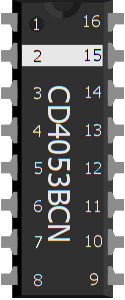
\includegraphics[width=.2\textwidth]{CD4053BCN_bb.png}};
\node[draw] at (0,5.5) {\textcolor{red}{1}};
\node[draw] at (0,4.8) {\textcolor{red}{2}};
\node[draw] at (0,4.1) {\textcolor{red}{3}};
\node[draw] at (0,3.4) {\textcolor{red}{4}};
\node[draw] at (0,2.7) {\textcolor{red}{5}};
\node[draw] at (0,2) {\textcolor{red}{6}};
\node[draw] at (0,1.3) {\textcolor{red}{7}};
\node[draw] at (0,0.6) {\textcolor{red}{8}};

\node[draw] at (3.1,5.5) {\textcolor{red}{16}};
\node[draw] at (3.1,4.8) {\textcolor{red}{15}};
\node[draw] at (3.1,4.1) {\textcolor{red}{14}};
\node[draw] at (3.1,3.4) {\textcolor{red}{13}};
\node[draw] at (3.1,2.7) {\textcolor{red}{12}};
\node[draw] at (3.1,2) {\textcolor{red}{11}};
\node[draw] at (3.1,1.3) {\textcolor{red}{10}};
\node[draw] at (3.1,0.6) {\textcolor{red}{9}};

\node[inner sep=0pt] (opamp) at (6,3)
{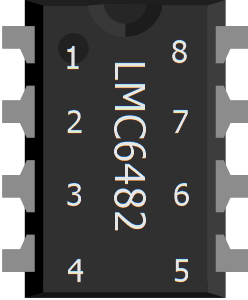
\includegraphics[width=.2\textwidth]{LMC6482AIN_bb.png}};

\node[draw] at (4.5,4.1) {\textcolor{blue}{1}};
\node[draw] at (4.5,3.4) {\textcolor{blue}{2}};
\node[draw] at (4.5,2.7) {\textcolor{blue}{3}};
\node[draw] at (4.5,2.0) {\textcolor{blue}{4}};

\node[draw] at (7.6,4.1) {\textcolor{blue}{8}};
\node[draw] at (7.6,3.4) {\textcolor{blue}{7}};
\node[draw] at (7.6,2.7) {\textcolor{blue}{6}};
\node[draw] at (7.6,2.0) {\textcolor{blue}{5}};

\node[inner sep=0pt] (opamp) at (12,3)
{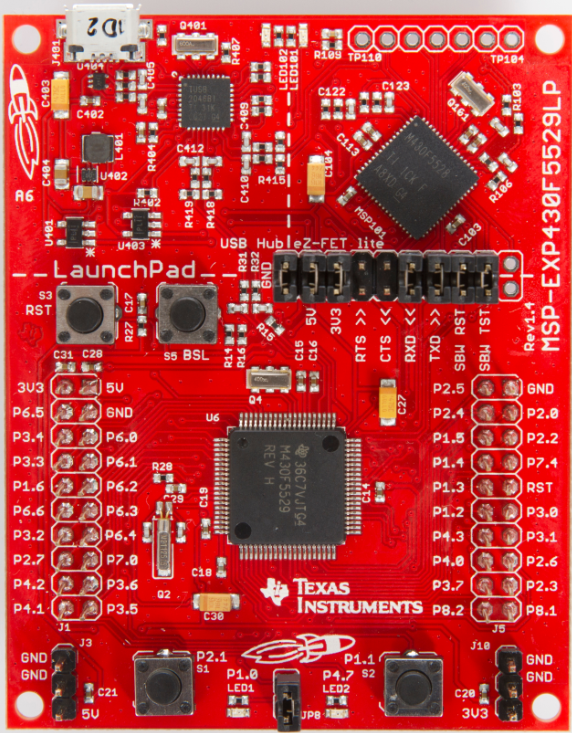
\includegraphics[width=.4\textwidth]{MSP430-USB-LP.PNG}};

\node[draw] at (9,2.7) {\textcolor{magenta}{5V}};
\node[draw] at (9,2) {\textcolor{magenta}{GND}};
\node[draw] at (9,1.3) {\textcolor{magenta}{P6.0}};
\node[draw] at (9,0.6) {\textcolor{magenta}{P6.1}};
\node[draw] at (9,-.1) {\textcolor{magenta}{P6.2}};

\node[draw] at (15,2.7) {\textcolor{magenta}{P2.5}};
%\draw[<->,thick] (russell.south east) -- (whitehead.north west)
%node[midway,fill=white] {Principia Mathematica};
\end{tikzpicture}

\end{document}